\vspace{-0.4cm}
Rodriguinho está muito animado com a empresa de serviços em TI que está abrindo.
Após já ter decidido o nome da empresa e o endereço onde o escritório será
instalado, Rodriguinho está agora definindo uma logomarca para a empresa.

Minimalista que é, ele decidiu que a logo consistirá apenas de um círculo
cortado por duas retas verticais, com a área entre elas pintadas de alguma cor
(a cor vai mudar a cada mês).

Para simplificar, considere que o círculo tem centro na origem do plano
cartesiano e tem raio $r$, e que as retas verticais cortam o eixo X nos
pontos $x_1$ e $x_2$. Como exemplo, a figura abaixo apresenta
uma logo com $r=5, x_1=-2, x_2=1$:

\vspace{-0.5cm}
\begin{center}
    %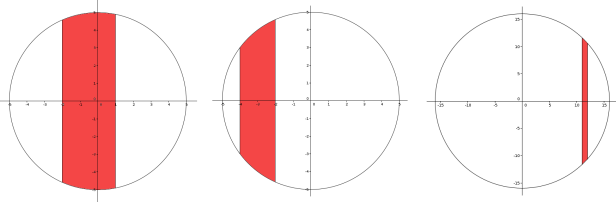
\includegraphics[scale=0.2]{logomarca/logomarca.pdf}
    \includegraphics[scale=0.3]{logomarca/logo1.png}
\end{center}

\vspace{-0.5cm}
Rodriguinho está preocupado com a quantidade de tinta que terá de comprar todos
os meses. Por isso, ele pediu sua ajuda para
determinar a área da região pintada na sua logomarca.


\subsection*{Entrada}

A única linha da entrada contém três inteiros $r$, $x_1$ e $x_2$
($1 \leq r \leq 50$, $-r \leq x_1 < x_2 \leq r$).

\subsection*{Saída}

Imprima uma linha contendo a área da região pintada, arredondada com três casas decimais.

\begin{table}[!h]
\centering
\begin{tabular}{|l|l|}
\hline
\begin{minipage}[t]{3in}
\textbf{Exemplo de entrada}
\begin{verbatim}
5 -2 1
\end{verbatim}
\vspace{1mm}
\end{minipage}
&
\begin{minipage}[t]{3in}
\textbf{Exemplo de saída}
\begin{verbatim}
29.386
\end{verbatim}
\vspace{1mm}
\end{minipage} \\
\hline
\end{tabular}
\end{table}

\begin{table}[!h]
\centering
\begin{tabular}{|l|l|}
\hline
\begin{minipage}[t]{3in}
\textbf{Exemplo de entrada}
\begin{verbatim}
5 -4 -2
\end{verbatim}
\vspace{1mm}
\end{minipage}
&
\begin{minipage}[t]{3in}
\textbf{Exemplo de saída}
\begin{verbatim}
15.729
\end{verbatim}
\vspace{1mm}
\end{minipage} \\
\hline
\end{tabular}
\end{table}

\begin{table}[!h]
\centering
\begin{tabular}{|l|l|}
\hline
\begin{minipage}[t]{3in}
\textbf{Exemplo de entrada}
\begin{verbatim}
16 11 12
\end{verbatim}
\vspace{1mm}
\end{minipage}
&
\begin{minipage}[t]{3in}
\textbf{Exemplo de saída}
\begin{verbatim}
22.233
\end{verbatim}
\vspace{1mm}
\end{minipage} \\
\hline
\end{tabular}
\end{table}
